%% LaTeX2e class for student theses
%% thesis.tex
%% 
%% Based on SDQ KIT Template by Erik Burger
%%
%% Karlsruhe Institute of Technology
%% Institute for Automation and Applied Informatics
%% AIDA Research Group
%%
%% Nicole Ludwig
%% nicole.ludwig@kit.edu
%%
%% Version 1.3, 20.11.2018

%% Available page modes: oneside, twoside
%% Available languages: english, ngerman
%% Available modes: draft, final
\documentclass[twoside, english,figuresleft]{thesisIAI}

%% ---------------------------------
%% | Additonal Packages |
%% ---------------------------------

% remove indentation throughout the document
\setlength{\parindent}{0pt}

\usepackage{tocbasic}

%%% Doc: ftp://tug.ctan.org/pub/tex-archive/macros/latex/contrib/caption/caption.pdf
\usepackage[tableposition=above]{caption}

% Aussehen der Captions
\captionsetup{
   margin = 10pt,
   font = {rm},
   labelfont = {bf},
   format = plain, % oder 'hang'
   indention = 0em,  % Einruecken der Beschriftung
   labelsep = space, %period, space, quad, newline
   justification = RaggedRight, % justified, centering, RaggedRight
   singlelinecheck = true, % false (true=bei einer Zeile immer zentrieren)
   position = bottom %top
}

%%% Bugfix Workaround
\DeclareCaptionOption{parskip}[]{}
\DeclareCaptionOption{parindent}[]{}

\usepackage{csquotes}
\usepackage{siunitx}

%% useful abreviations

\newcommand\ie{i.\,e.\xspace}
\newcommand\eg{e.\,g.\xspace}
\newcommand\Eg{E.\,g.\xspace}
\newcommand\NB{N.\,B.\xspace}
\newcommand\BSc{B.\,Sc.\xspace}
\newcommand\MSc{M.\,Sc.\xspace}
\newcommand\PhD{Ph.\,D.\xspace}
\newcommand\etc{etc.\xspace}
\newcommand\cf{cf.\xspace}
\newcommand\Cf{Cf.\xspace}
\newcommand\etal{et\,al.\xspace}
\newcommand\page[1]{p.\,#1}
\newcommand\pages[1]{pp.\,#1}
\newcommand\ham{a.\,m.\xspace}
\newcommand\hpm{p.\,m.\xspace}
	
\newcommand\zB{z.\,B.\xspace}
\newcommand\proz{\,\%\xspace}

%% Useful definitions for tables --------------------------------------------------------- %% 

% um Tabellenspalten mit Flattersatz zu setzen, muss \\ vor
% (z.B.) \raggedright geschuetzt werden:
\newcommand{\PreserveBackslash}[1]{\let\temp=\\#1\let\\=\temp}

% Linksbuendig:
\newcolumntype{v}[1]{>{\PreserveBackslash\RaggedRight\hspace{0pt}}p{#1}}
\newcolumntype{M}[1]{>{\PreserveBackslash\RaggedRight\hspace{0pt}}m{#1}}
\newcolumntype{Y}{>{\PreserveBackslash\RaggedLeft\hspace{0pt}}X}
%%% Spalten fuer Mathematik
%
% serifenlose Matheschrift
%\newcolumntype{s}[1]{%
%  >{\DC@{.}{,}{#1}\mathsf\bgroup}l%
%  <{\egroup\DV@end}%
%}

% Tabellenspaltentyp fuer den Kopf: (Farbe + Ausrichtung)
\newcolumntype{H}[1]{>{\columncolor{tableheadcolor}}l}

%%% ---|Layout der Tabellen |-------------------

% Neue Umgebung fuer Tabellen:

\newenvironment{Tabelle}[2][c]{%
  \tablestylecommon
  \begin{longtable}[#1]{#2}
  }
  {\end{longtable}%
  \tablerestoresettings
}

% Groesse der Schrift in Tabellen
\newcommand{\tablefontsize}{ \footnotesize}
\newcommand{\tableheadfontsize}{\footnotesize}

% Layout der Tabelle: Ausrichtung, Schrift, Zeilenabstand
\newcommand\tablestylecommon{%
  \renewcommand{\arraystretch}{1.4} % Groessere Abstaende zwischen Zeilen
  \normalfont\normalsize            %
  \sffamily\tablefontsize           % Serifenlose und kleine Schrift
  \centering%                       % Tabelle zentrieren
}

\newcommand{\tablestyle}{
  \tablestylecommon
  %\tablealtcolored
}

% Ruecksetzten der Aenderungen
\newcommand\tablerestoresettings{%
  \renewcommand{\arraystretch}{1}% Abstaende wieder zuruecksetzen
  \normalsize\rmfamily % Schrift wieder zuruecksetzen
}

% Tabellenkopf: Serifenlos+fett+schraeg+Schriftfarbe
\newcommand\tablehead{%
  \tableheadfontsize%
  \sffamily\bfseries%
  %\slshape
  %\color{white}
}

\newcommand\tablesubheadfont{%
  \tableheadfontsize%
  \sffamily\bfseries%
  \slshape
  %\color{white}
}

\newcommand\tableheadcolor{%
  %\rowcolor{tablesubheadcolor}
  %\rowcolor{tableblackheadcolor}
  \rowcolor{tableheadcolor}%
}

\newcommand\tablesubheadcolor{%
  \rowcolor{tablesubheadcolor}
  %\rowcolor{tableblackheadcolor}
}

\newcommand{\tableend}{\arrayrulecolor{black}\hline}

% Tabellenkopf (1=Spaltentyp, 2=Text)
% \newcommand{\tablehead}[2]{
%   \multicolumn{1}{#1@{}}{%
%     \raisebox{.1mm}{% Ausrichtung der Beschriftung
%       #2%
%     }\rule{0pt}{4mm}}% unsichtbare Linie, die die Kopfzeile hoeher macht
% }


\newcommand{\tablesubhead}[2]{%
  \multicolumn{#1}{>{\columncolor{tablesubheadcolor}}l}{\tablesubheadfont #2}%
}

% Tabellenbody (=Inhalt)
\newcommand\tablebody{%
\tablefontsize\sffamily\upshape%
}

\newcommand\tableheadshaded{%
  \rowcolor{tableheadcolor}%
}
\newcommand\tablealtcolored{%
  \rowcolors{1}{tablerowcolor}{white!100}%
}
%%% --------------------------------------------

\usepackage{ragged2e}

%% Rotate table head
%% http://tex.stackexchange.com/questions/98388/how-to-make-table-with-rotated-table-headers-in-latex
%% http://tex.stackexchange.com/questions/32683/rotated-column-titles-in-tabular
\newcommand*\rottblhead{\rotatebox{75}}

\usepackage{cleveref}
%\usepackage[utf8]{inputenc}

\usepackage[nosuper,toc,acronyms]{glossaries}
\usepackage{url}
\usepackage{eso-pic}
\usepackage{caption}
\usepackage{subcaption}
\usepackage{makecell}
\usepackage{tabularx}
\usepackage{float}

\newcolumntype{L}{>{\raggedright\arraybackslash}X}

\newcommand\BackgroundPic{%
\put(0,0){%
\parbox[b][\paperheight]{\paperwidth}{%
\vfill
\centering
\includegraphics[width=\paperwidth,%
keepaspectratio]{logos/bulb.png}%
\vfill
}}}

\newcommand{\tcite}{\Textcite}
\newcommand{\acrs}{\acrshort}

\NewDocumentCommand{\apply}{O{,~}mm}
{% #1 = output separator, #2 = command to apply, #3 = list
  \critch_apply:Nnn { #2 } { #1 } { #3 }
}

%% ---------------------------------
%% | Information about the thesis  |
%% ---------------------------------

%% Name of the author
\author{Marcel Herm}

%% Title (and possibly subtitle) of the thesis
%\title{GIS meets energy}
\title{Evaluating the benefit of grid-based weather information in energy forecasting}

%% Type of the thesis 
\thesistype{Bachelors's Thesis}
%\thesistype{Seminar Paper}

%% Change the faculty here
%\faculty{Seminar}
%\faculty{Engineering}
\faculty{Informatics}
%\faculty{Economics}

%% The advisors are PhDs or Postdocs
\advisorone{Nicole Ludwig, M.Sc}
%% The second advisor can be omitted
\advisortwo{Marian Turowski, M.Sc}

%% Please enter the start end end time of your thesis
\editingtime{2019/07/01}{2019/10/31}

\settitle

%% Please do not change anything in this tex file without talking to your supervisor
%% LaTeX2e class for student theses
%% format.tex
%% 
%% Based on SDQ KIT Template by Erik Burger
%%
%% Karlsruhe Institute of Technology
%% Institute for Automation and Applied Informatics
%% AIDA Research Group
%%
%% Nicole Ludwig
%% nicole.ludwig@kit.edu
%%
%% Version 1.2.1, 2018-10-11

%% This file switches between the official reviewers and addresses of the faculties 

\ifthenelse{\equal{\thefaculty}{Seminar}}{\uppertitleback}{
	\ifthenelse{\equal{\thefaculty}{Engineering}}{\uppertitleback{Karlsruher Institut für Technologie\\ Fakultät für Maschinenbau\\ Postfach 6980\\ 76128 Karlsruhe}}{
		\ifthenelse{\equal{\thefaculty}{Informatics}}{\uppertitleback{Karlsruher Institut für Technologie\\ Fakultät für Informatik\\ Postfach 6980\\ 76128 Karlsruhe}}{\uppertitleback{Karlsruher Institut für Technologie \\ Fakultät für Wirtschaftswissenschaften \\ Kollegiengebäude am Kronenplatz \\ Geb. 05.20, 3. OG, Raum 3C-05 \\ 76133 Karlsruhe}}}}

\ifthenelse{\equal{\thefaculty}{Informatics}}{\reviewerone{Prof. Dr. Veit Hagenmeyer}}{\reviewerone{apl. Prof. Dr. Ralf Mikut}}

\ifthenelse{\equal{\thefaculty}{Seminar}}{\reviewertwo{}}{
	\ifthenelse{\equal{\thefaculty}{Informatics}}{\reviewertwo{Prof. Dr. Achim Streit}}{
		\ifthenelse{\equal{\thefaculty}{Engineering}}{\reviewertwo{Prof. Dr. Veit Hagenmeyer}}{\reviewertwo{Prof. Dr. Wolf Fichtner}}}}

\ifthenelse{\equal{\thefaculty}{Seminar}}{\facultyname{Energy Informatics Seminar}}{
	\ifthenelse{\equal{\thefaculty}{Engineering}}{\facultyname{\iflanguage{english}{at the Department of Mechanical Engineering}{an der Fakultät für Maschinenbau}}}{
		\ifthenelse{\equal{\thefaculty}{Informatics}}{\facultyname{\iflanguage{english}{at the Department of Informatics}{an der Fakultät für Informatik}}}{
		\facultyname{\iflanguage{english}{at the Department of Economics and Management}{an der Fakultät für Wirtschaftswissenschaften}}}}}
		
		
		




%% --------------------------------
%% | Settings for word separation |
%% --------------------------------

%% Describe separation hints here.
%% For more details, see 
%% http://en.wikibooks.org/wiki/LaTeX/Text_Formatting#Hyphenation
\hyphenation{
% me-ta-mo-del
}

%% --------------------------------
%% | Bibliography                 |
%% --------------------------------

% Please make sure your bibfiles name is thesis.bib and is located in the tex subfolder
\usepackage[                 % !! what about the ``biblatex.cfg''?
        backend=bibtex8,      % (bibtex), bibtex8, biber
%        %
        style=authoryear,		 %numeric-comp,
%        bibstyle=,          % should not be used without citestyle and vice versa
%        citestyle=,
%        natbib=true,
        %
%        sorting=nty,        % (nty), nyt, nyvt, anty, anyt, anyvt, debug, none
%        sortlos=los,        % bib, (los)
%        sortcites=false,    % false
%        maxnames=2,         % <integer> (3)
				maxcitenames=2,      % sets the maximum numbers of authors before abbreviated to et al in text
				maxbibnames=25,       % sets the maximum numbers of authors before abbreviated to et al in bibliography
%        minnames=1,         % (1)
%        maxitems=3,         % (3)
%        minitems=1,         % (1)
%        autocite=,          % inline, footnote, superscript, ...
%        autopunct=true,     % true
%        babel=none,         % (none), hyphen, other, other*
%        block=none,         % (none), space, par, nbpar, ragged
        hyperref=true,      % false
%        backref=false,      % false
%        indexing=false,     % true, (false), cite, bib
%        refsection=none,    % (none), part, chapter, section, subsection
%        refsegment=none,    % (none), part, chapter, section, subsection
%        citereset=none,     % (none), part, chapter, section, subsection
%        abbreviate=true,    % true
%        date=long,          % short, (long)
%        urldate=short,      % (short), long
%        defernums=false,    % false
%        punctfont=false,    % false
        %
%        mincrossrefs=2,     % 2
        bibencoding=inputenc,   % (ascii), inputenc, <encoding>
        %%
%        keywsort=false,     % false
    %
%     useauthor=false,   % true
%     useeditor=false,   % true
%        useprefix=true,     % false
    %
%        pagetracker=true,   % true, (false), page, spread
%     citetracker=true,   % true, (false), context, strict, constrict
%     ibidtracker=true,   % true, (false), context, strict, constrict
%     opcittracker=true,   % true, (false), context, strict, constrict
%     loccittracker=true, % true, (false), context, strict, constrict
%        terseinits=true,    % false
%     labelalpha=true,   % false
%     labelnumber=true,   % false
%     labelyear=true,   % false
%     singletitle=true,   % false
      uniquename=init,   % true, (false), init
%
        doi=false,
        url=false,
				isbn = false,
        giveninits = true % render first/middle names as initals
            ]{biblatex}
	
\makeatletter
\def\blx@maxline{77}
\makeatother
	
	\bibliography{tex/thesis}
   
      %  \DefineBibliographyStrings{ngerman}{%
         %   bibliography     = {Literaturverzeichnis},  % = \bibname
         %   references       = {Literatur},             % = \refname
     %   }
        \defbibnote{alphabetic}{%
            Die Literaturangaben sind alphabetisch nach den Namen
            der Autoren sortiert. Bei mehreren Autoren wird nach
            dem ersten Autor sortiert.\par
            Und mit dem neuen \LPack{biblatex}-Paket funktioniert
            das auch, wie man unschwer erkennen kann.\par\bigskip
        }

% -------------------------------------------------------------------------------------------------
%% declare author names as "last, first".
%% Either for the first author only or for all authors
%\DeclareNameFormat{author}{%
%    \ifthenelse{\value{listcount}=1}
%        {#1%                                            % first author
%            \ifblank{#3}{}{\addcomma\space #3}}
%        {#1%                                            % all the other authors (last, first)
%            \ifblank{#3}{}{\addcomma\space #3}}%
%%        {\ifblank{#3}{}{#3\space}%                      % all the other authors (first last)
%%            #1}%
%    \ifthenelse{\value{listcount}<\value{liststop}}
%        {,\space}
%            {}
%}
%
%%http://projekte.dante.de/DanteFAQ/BiblatexReihenfolgeAutoren
%\DeclareNameFormat{last-first}{%
%  \iffirstinits
%    {\usebibmacro{name:last-first}{#1}{#4}{#5}{#7}}
%    {\usebibmacro{name:last-first}{#1}{#3}{#5}{#7}}%
%  \usebibmacro{name:andothers}}
%\DeclareNameFormat{labelname}{%
%   \ifuseprefix
%     {\usebibmacro{name:last-first}{#1}{#4}{#5}{#8}}
%     {\usebibmacro{name:last-first}{#1}{#4}{#6}{#8}}%
%   \usebibmacro{name:andothers}}

%  \DefineBibliographyStrings{english}{%
%    typeeditor = {{}{}},
%    typeeditors = {{}{}},
%    in = {{}{}},
%    inseries = {{}{}},
%    byeditor = {{}{}}
%  }

%-------------------------------------------------------------------------------------------------

%% http://www.golatex.de/biblatex-anpassen-die-x-te-frage-t4657.html
\renewbibmacro*{journal+issuetitle}{%
  \usebibmacro{journal}%
  \setunit*{\addcomma\space}%
  \iffieldundef{series}
    {}
    {\newunit
     \printfield{series}%
     \setunit{\addcomma\space}}%
  \printfield{volume}%
  \setunit*{\addcomma\space}%
  \printfield{number}%
  \setunit{\addcomma\space}%
  \printfield{eid}%
  \setunit{\addspace}%
  \usebibmacro{issue+date}%
  \setunit{\addcolon\space}%
  \usebibmacro{issue}%
  \newunit}

\DeclareFieldFormat[article]{volume}{\bibstring{jourvol}~#1}
\DeclareFieldFormat[article]{number}{\bibstring{number}~#1} 
%\DeclareFieldFormat[article]{edition}{\bibstring{edition}~#1} 

%% http://mrunix.de/forums/showthread.php?t=67386
\DefineBibliographyStrings{english}{jourvol={Vol\adddot}} 
\DefineBibliographyStrings{english}{number={No\adddot}} 
\DefineBibliographyStrings{english}{edition={Ed\adddot}} 

\AtBeginBibliography{%
  % Setzt die Autoren-Vornamen auf Kapit�lchen 
  \renewcommand*{\mkbibnamefirst}{\textsc}
  \renewcommand*{\mkbibnamelast}{\textsc}
  \renewcommand*{\mkbibnameprefix}{\textsc}
  \renewcommand*{\mkbibnameaffix}{\textsc}
  
  %%Doppelpunkt nach Namen, kein Punkt
  %\renewcommand*{\labelnamepunct}{\addcolon\space} 
  
  \DeclareFieldFormat{name}{\textsc{#1\isdot}}
  \DeclareFieldFormat{title}{\mkbibemph{#1\isdot}}
  
  %%\DeclareFieldFormat[article]{title}{#1}
  %%\DeclareFieldFormat[article]{title}{\mkbibquote{#1}}
  \renewcommand*{\mkbibquote}[1]{\mkbibemph{#1\isdot}}
 
  % http://tex.stackexchange.com/ ...
  % questions/16716/spell-out-volume-and-edition-in-words-biblatex-in-german
  %\renewcommand*{\mkbibordedition}[1]{\Ordinalstringnum{#1}[f]}
  \renewcommand*{\mkbibordedition}[1]{\ordinalnum{#1}}
} 

%% --------------------------------
%% | Glossary                     |
%% --------------------------------
\makeglossaries

%\newglossaryentry{ECMWF}
%{
%  name=European Centre of Medium-Range Weather Forecasts,
%  description={a research institute and a 24/7 operational service, producing global numerical weather predictions and other data}
%}

% \newacronym{}{}{}

% data sources
\newacronym{ecmwf}{ECMWF}{European Centre of Medium-Range Weather Forecasts}
\newacronym{nuts}{NUTS}{Nomenclature des Unités territoriales statistiques}
\newacronym{sdhws}{SDHWS}{Solar Domestic Hot Water Systems}
\newacronym{epex}{EPEX SPOT}{European Power Exchange}
\newacronym{dwd}{DWD}{Deutscher Wetterdienst}
\newacronym{silo}{SILO}{Scientific Information for Land Owners}
\newacronym{hc3}{HC3}{Helioclim-3}
\newacronym{mm5}{MM5}{Fifth-generation Mesoscale Model}
\newacronym{wrf}{WRF}{Weather Research and Forecasting Model}
\newacronym{noaaesrl}{NOAA/ESRL}{National Oceanic and Atmospheric Administration - Earth System Research Laboratory}

% error measures
\newacronym{rmse}{RMSE}{Root-Mean-Square Error}
\newacronym{mape}{MAPE}{Mean Absolute Percentage Error}

% neural networks
\newacronym{nn}{NN}{Neural Networks}
\newacronym{wnn}{WNN}{Wavelet Neural Networks}

% regression
\newacronym{lr}{LR}{Linear Regression}
\newacronym{sslr}{SSLR}{Simple Seasonal Linear Regression}
\newacronym{qr}{QR}{Quantile Regression}
\newacronym{mlr}{MLR}{Multiple Linear Regression}
\newacronym{svm}{SVM}{Support Vector Machines}
\newacronym{svr}{SVR}{Support Vector Regression}
\newacronym{mars}{MARS}{Multivariate Adaptive Regression Splines}

% autoregressive
\newacronym{ar}{AR}{Autoregressive}
\newacronym{ma}{MA}{Moving Average}
\newacronym{arma}{ARMA}{Autoregressive-Moving Average}
\newacronym{armax}{ARMAX}{Autoregressive-Moving Average with Exogenous Inputs}
\newacronym{arima}{ARIMA}{Autoregressive Integrated Moving Average}
\newacronym{arimax}{ARIMAX}{Autoregressive Integrated Moving Average with Exogenous Inputs}
\newacronym{cards}{CARDS}{Coupled Autoregressive and Dynamical System}
\newacronym{arwd}{ARWD}{Autoregressive model using an average weekly profile}
\newacronym{arwdy}{ARWDY}{Autoregressive model using an average weekly profile including annual seasonality}

%\newacronym{ma}{MA}{Moving Average}


% kriging
\newacronym{ok}{OK}{Ordinary Kriging}
\newacronym{ck}{CK}{Co-Kriging}
\newacronym{rk}{RK}{Regression Kriging}

% ensemble methods
\newacronym{anen}{AnEn}{Analog Ensemble}
\newacronym{ecmwfeps}{ECMWF-EPS}{ECMWF Ensemble Prediction System}
\newacronym{leps}{LEPS}{Limited-area Ensemble Prediction System}

% genetic
\newacronym{gga}{GGA}{Grouping Genetic Algorithm}
\newacronym{rf}{RF}{Random Forests}

% dimensionality reduction
\newacronym{pca}{PCA}{Principal Component Analysis}

% other methods
\newacronym{pdf}{PDF}{Probability Density Function}
\newacronym{elm}{ELM}{Extreme Learning Machine}
\newacronym{cro}{CRO}{Coral Reefs Optimization}
\newacronym{gam}{GAM}{Generalized Additive Models}
\newacronym{mos}{MOS}{Model Output Statistics}
\newacronym{emos}{EMOS}{Ensemble Model Output Statistics}
\newacronym{idw}{IDW}{Inverse Distance Weighting}
\newacronym{rams}{RAMS}{Regional Atmospheric Modelling System}
\newacronym{lasso}{LASSO}{Least Absolute Shrinkage Selection Operation}
\newacronym{kde}{KDE}{Kernel Density Estimation}
\newacronym{hwt}{HWT-ESM}{Holt-Winters-Taylor Exponential Smoothing Method}
\newacronym{vd}{VD}{Variance Deficit}
\newacronym{pe}{PE}{Persistence Ensemble}


% others
\newacronym{pv}{PV}{photovoltaic}
\newacronym{ghi}{GHI}{Global Horizontal Solar Irradiance}
\newacronym{c3s}{C3S}{Copernicus Climate Change Service}



%% ====================================
%% ====================================
%% ||                                ||
%% || Beginning of the main document ||
%% ||                                ||
%% ====================================
%% ====================================
\begin{document}

%\AddToShipoutPicture*{\BackgroundPic}

\hypersetup{pageanchor=false}

%% Set PDF metadata
\setpdf

%% Set the title
\maketitle

%% The Preamble begins here
\frontmatter

%% LaTeX2e class for student theses: Declaration of independent work
%% sections/declaration.tex
%% 
%% Karlsruhe Institute of Technology
%% Institute for Program Structures and Data Organization
%% Chair for Software Design and Quality (SDQ)
%%
%% Dr.-Ing. Erik Burger
%% burger@kit.edu
%%
%% Version 1.3.2, 2017-08-01

\thispagestyle{empty}
\null\vfill
\noindent\hbox to \textwidth{\hrulefill} 
\iflanguage{english}{I declare that I have developed and written the enclosed
\ifthenelse{\equal{\thefaculty}{Engineering}}{thesis}{\ifthenelse{\equal{\thefaculty}{Informatics}}{thesis}{paper}} completely by myself, and have not used sources or means without
declaration in the text.}%
{Ich versichere wahrheitsgemäß, die Arbeit
selbstständig angefertigt, alle benutzten Hilfsmittel vollständig und genau
angegeben und alles kenntlich gemacht zu haben, was aus Arbeiten anderer
unverändert oder mit Änderungen entnommen wurde.}
 
 
%% ---------------------------------------------
%% | Replace PLACE and DATE with actual values |
%% ---------------------------------------------
\textbf{PLACE, DATE}
\vspace{1.5cm}
 
\dotfill\hspace*{8.0cm}\\
\hspace*{2cm}(\theauthor) 
\cleardoublepage

\setcounter{page}{1}
\pagenumbering{roman}

%% ----------------
%% |   Abstract   |
%% ----------------
 
%% For theses written in English, an abstract both in English
%% and German is mandatory.
%%
%% Seminar Papers written in English need only an English abstract.
%%
%% For theses written in German, a German abstract is sufficient.
%%
%% The text is included from the following files:
%% - sections/abstract
%% - sections/zusammenfassung

\chapter*{Acknowledgements}

Firstly, I would like to express my sincere gratitude to Nicole Ludwig, who elaborated the subject of this thesis, and Marian Turowski, who assisted her supervising this thesis. Their professional and incredibly considerate supervision were extremely helpful for me throughout the last few months.\\

To Prof. Dr. Veit Hagenmeyer, I am most grateful for giving me the chance to complete my thesis at IAI.\\

Further, I would like to thank Kaleb Phipps, who provided some very useful code, saving me a lot of time that would have otherwise been spent for debugging due to issues in the implementation phase.\\

In addition, I am deeply indebted to Janine von Hodenberg for her enduring assistance and helpful consultancy.\\

And finally, eternal thanks goes to my family, supporting me throughout many years without ever questioning or doubting me.\\



\pdfbookmark[1]{Abstract}{Abstract}

\chapter*{Abstract}

\begin{center}
  \begin{minipage}{12cm}
    \begin{sloppypar}
		As the share of electricity from regenerative sources is growing constantly, the weather becomes an increasingly important factor in the analysis of electricity markets. Hence, this thesis uses local weather data to predict electricity spot prices. More precisely, we include wind speed and temperature from individual German weather stations into time series and statistical learning models. However, as the available weather information is vast and renewable power is not generated everywhere, we use random forests and Bayesian structural time series to perform a feature selection. Overall, we manage to improve our forecasting accuracy of the EPEX electricity prices by up to \SI{7.69}{\percent} in terms of root mean squared error and up to \SI{8.19}{\percent} in terms of mean absolute error.
    \end{sloppypar}
  \end{minipage}
\end{center}

\hypersetup{pageanchor=true}
%% ------------------------
%% |   Table of Contents  |
%% ------------------------
\tableofcontents
\listoffigures
\listoftables

%% -----------------
%% |   Main part   |
%% -----------------

\mainmatter

\chapter{Introduction}
\label{ch:Introduction}

According to \tcite{Li2009}, weather has a great impact on electricity demand. So it is not surprising, that several works, such as \tcite{Bofinger2006} and \tcite{Sperati2016}, use weather data to improve forecasts of energy-related quantities. How to best use grid-based weather data for energy forecasting is an important problem. This is why Nicole Ludwig issued this subject, that has not been covered yet by others. In the near future, the dependence of electricity demand on the current weather is expected to increase even further, as the share of electricity generation from renewable resources also increases. Potentially deployed functions of the future, such as \gls{dsm}, will play their part to do so, too. It is notable, that works which use non-gridded data, often do some sort of interpolation, which is not necessary for grid-based data that already is equidistantly distributed and, thus, requires less effort. Also, grid-based data often is available over large areas, which means, that there is less limitation of locality and thus more general predictions are possible with a higher quality of data. The fact that this subject has not been covered yet by others, may relate to the issue that it was still more complicated to acquire grid-based data than station-based in the past few years. However, since 2018, the Copernicus Climate Change Service (C3S) offers easy access to grid-based data. Additionally, their API gets updated frequently and therefore, access gets more comfortable with time, making the issue of how to best use grid-based weather data even more relevant.\\

The structure of this thesis continues in the following manner. \Cref{ch:RW} gives an overview of similar works. \Cref{ch:methods} will present the used methods. Then, in \Cref{ch:Evaluation}, the overall approach will be explained and elaborated results will be presented. Finally, in \Cref{ch:discussion} and \Cref{ch:Conclusion}, the results will be first critically inspected, important insights will be outlined and finally, an outlook for further research will be given.\\

%TODO mention that the idea for this thesis originated from Nicole Ludwig\footnote{\url{https://www.iai.kit.edu/2154_2161.php}}\label{ack:nicole}\\
%
%TODO mention \gls{dsm} somewhere\\
%
%According to \tcite{Li2009}, especially temperature and perceived temperature have a great impact on energy demand. Consequently, several authors combine forecasting energy time series using weather data. They mostly either focus on forecasting \gls{pv} electricity generation as in \tcite{Bofinger2006} and \tcite{Sperati2016} or on electricity generation from wind as in \tcite{Davo2016} and \tcite{Alessandrini2015}.\\
%
%It is notable, that works using station-based data often try to do some sort of geographic interpolation to be able to obtain values for every possible position. Considering this thesis, there is no such problem, as the used grid-based data already provides such distributed values. Thus, when using grid-based data, the step of interpolation can be omitted, and therefore, less effort is required. Some works also regard only forecasting for specific locations or accumulated values for bigger areas. With grid-based data, more general predictions can be made regarding the target location, as there is no binding to a certain locality.\\
%
%Another interesting point is, that the works that forecast weather related time series all used grid-based data, though some of them also used station-based data to refine their forecasts. Among the papers that aimed for forecasting power or similar often only station-based data is used which leads to the assumption that less effort has been made in these fields, as it is still more complex to acquire grid-based data. However, there remains the possibility that station-based data is more suitable, even though this means a trade-off in terms of flexibility. Of course it is also possible that this has to do with the fact, that there is no grid-based power data available as this may harm privacy issues.\\

%Your thesis should start with an introduction. The introduction is supposed to motivate your thesis.
%Discuss the relevance of your topic, why are you looking into it, why is it relevant in the field? Cite important research related to your motivation.
%Briefly state the problem as in the abstract and repeat the contribution, for example in the form of research questions. 

%Give an outline of your thesis.


%Below, you will find an example figure (\Cref{fig:example}). Please use the caption of your figures to describe everything in the figure, additionally to what you have written about the figure in the text. Everyone should be able to understand the figure just reading its caption.

%\begin{figure}[h!]%
%\centering
%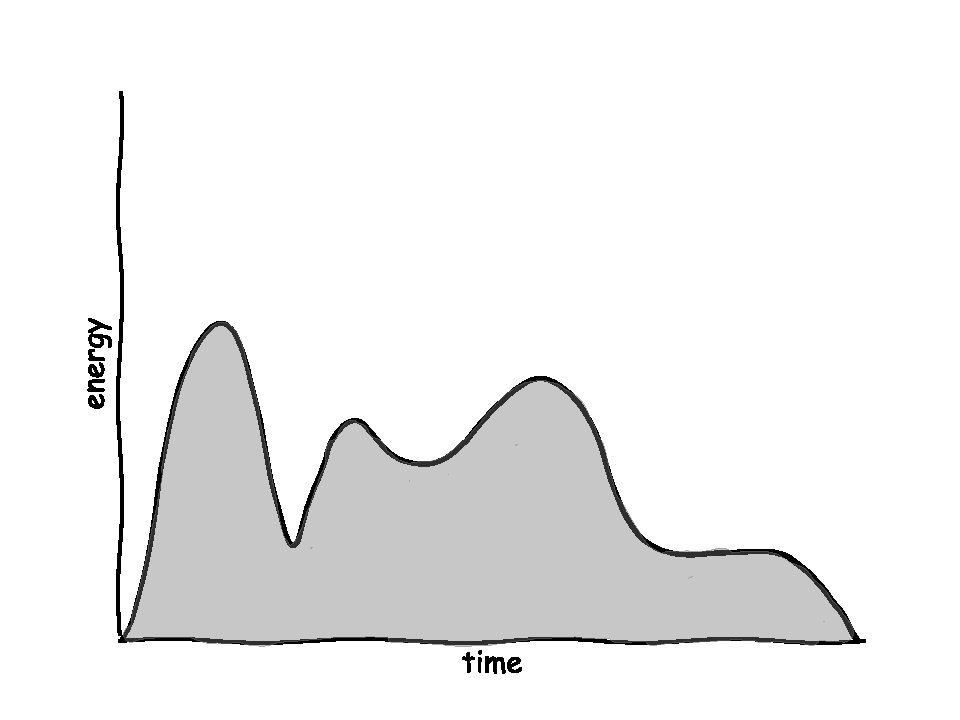
\includegraphics[width=0.5\columnwidth]{plots/Figure_2_demand}%
%\caption{This is an example figure. It shows a fictional demand of energy (in grey) over time.}%
%\label{fig:example}%
%\end{figure}

%This work is supposed to refer about including grid-based data into load forecasts using different methods.\\

\chapter{Related Work}
\label{ch:RW}

This chapter is supposed to summarise previous work of other researchers related to your topic.
The aim is to give an overview of existing literature while highlighting differences and similarities to this thesis.

Please choose a coherent citation style throughout the thesis. For example

\begin{itemize}
	\item Direct citation of results, an approach or similar
	\item[] \Textcite{Fan.2015} find that their method improves the benchmark.
	\item Indirect citation
	\item[] Recent research highlights the importance of this method \Parencite{Fan.2015}.
	\item Direct citation
	\item[] \textquote{\emph{Energy optimisation in buildings is important}} \Parencite{Fan.2015}.
\end{itemize}




\chapter{Methodology}
\label{ch:methods}

%This chapter should introduce to the theoretical background of your thesis. Any method you use to obtain the results later should be introduced and explained. 

Using weather data from ECMWF Copernicus Climate Change Service (C3S).\\
Using load data from \url{https://data.open-power-system-data.org/}.\\
First downloaded whole Datasets from 2006-2019, but as the load for germany is properly available since 2015, now reduced dataset to 2015-2019.\\
Also checked for non-existing values, only 2 last timestamps values for the load are missing.\\

\section{Method 1}

Maybe use Random Forests for variable selection as in Nicoles paper? \cite{Ludwig2015}\\

%This is an example for a simple equation without equation numbering.
%$$
%\sum\limits_{i=1}^{n}{x_i}
%$$

You can also use equation numbering if you need to refer to an equation later \eg \Cref{eq:ex1}.


\begin{equation}
a^2 + b^2 = c^2
\label{eq:ex1}
\end{equation}

Additionally, simple equations can be put inline with the text, for example, $x \in X$. Remember to set all variables in math font \ie all $x$, $i$ and so on.

\section{Method 2}

\dots


\chapter{Evaluation}
\label{ch:Evaluation}

\section{Data}
\label{sec:data}

Of course choosing data sources as well as sorting and cleaning the data also requires a certain amount of time and effort. Thus it will be explained hereinafter how this has been done for the data used in this thesis.

\subsection{ECMWF}

The data used in this thesis originates from \acrshort{ecmwf}, which is a research institute that produces global numerical weather predictions and other data.\\
It is time series based and for each timestamp there is a 2-dimensional array referred to by longitude and latitude respectively.\\

It must be mentioned that, as the data used has been reanalized, so the expected error is likely to be smaller than if working with real-time data.\\

As data parameters there are also longitude and latitude, where the longitude is chosen to be from 5.5 to 15.5 and the latitude from 47 to 55.5. As the resolution of the used grid is at 0.25°, this results in a total of 1435 grid points per timestamp. As the range of the data from \acrshort{ecmwf} extends from 2015/1/1 to 2019/3/31(TODO update), there is a total of 1551 days with each 12 timestamps due to the 2 hours frequency and thus 18612 timestamps. Considering that there is a value for each point in the grid and every timestamp, there are 26708220 values for each variable.\\

In order to reduce complexity, a shapefile of the \acrshort{nuts} dataset was used. The shapefile contains all countries in the EU. The shape of germany was filtered from this data and each point in the \acrshort{ecmwf} dataset is checked wether it is within germany or not. The result can be seen in figure \ref{fig:isin}.\\

\subsection{Population}



\begin{figure}[h!]%
\centering
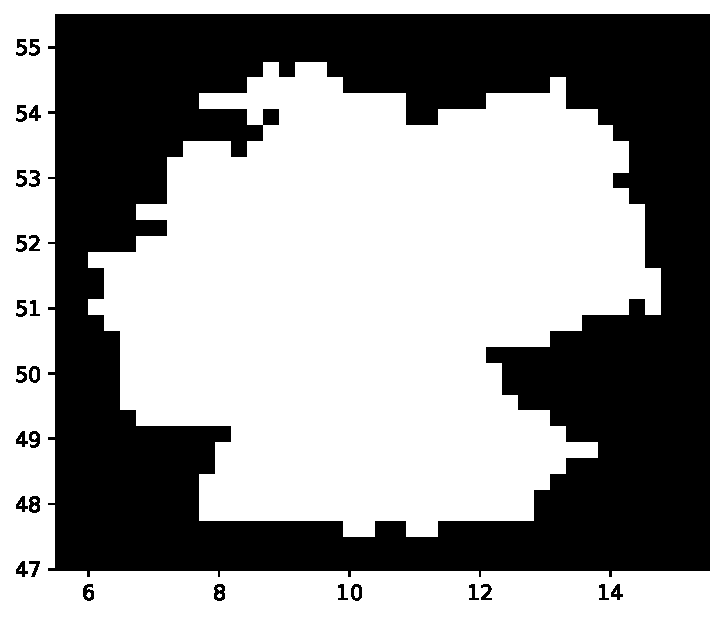
\includegraphics[width=0.8\textwidth]{plots/isin}%
\caption{2D boolean numpy.ndarray used to filter grid squares that are within germany. It was created by using a shapefile of germany (TODO insert source \url{https://ec.europa.eu/eurostat/cache/GISCO/distribution/v2/nuts/nuts-2016-files.html}) and checking for each point of the grid if it is within the shapefile. (TODO shorter explanation, put explanation in text)}%
\label{fig:isin}%
\end{figure}

\begin{figure}[h!]%
\centering
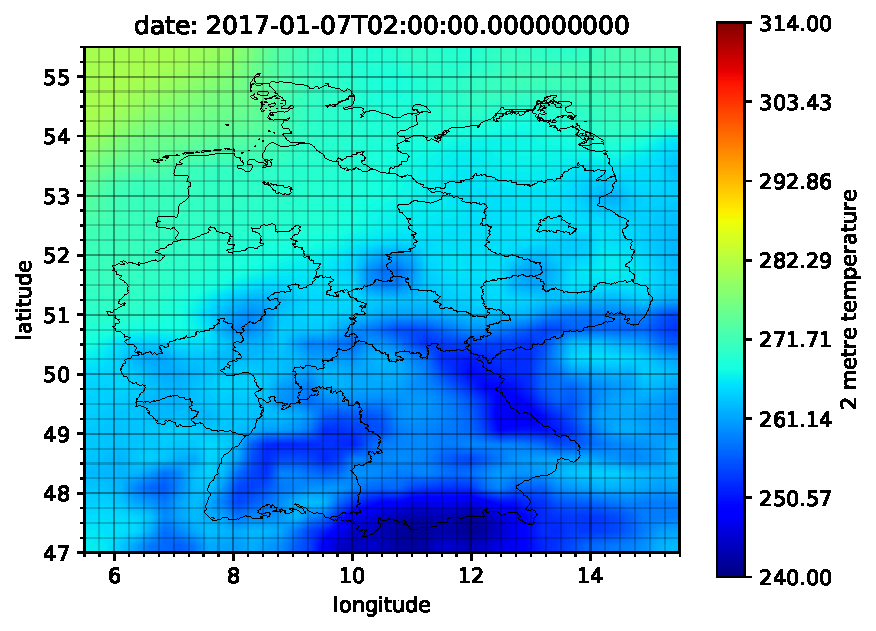
\includegraphics[width=\textwidth]{plots/0_2017010702_20190617161317}%
\caption{Map showing day with lowest temperature in germany.}%
\label{fig:0_2017010702_20190617161317}%
\end{figure}

\begin{figure}[h!]%
\centering
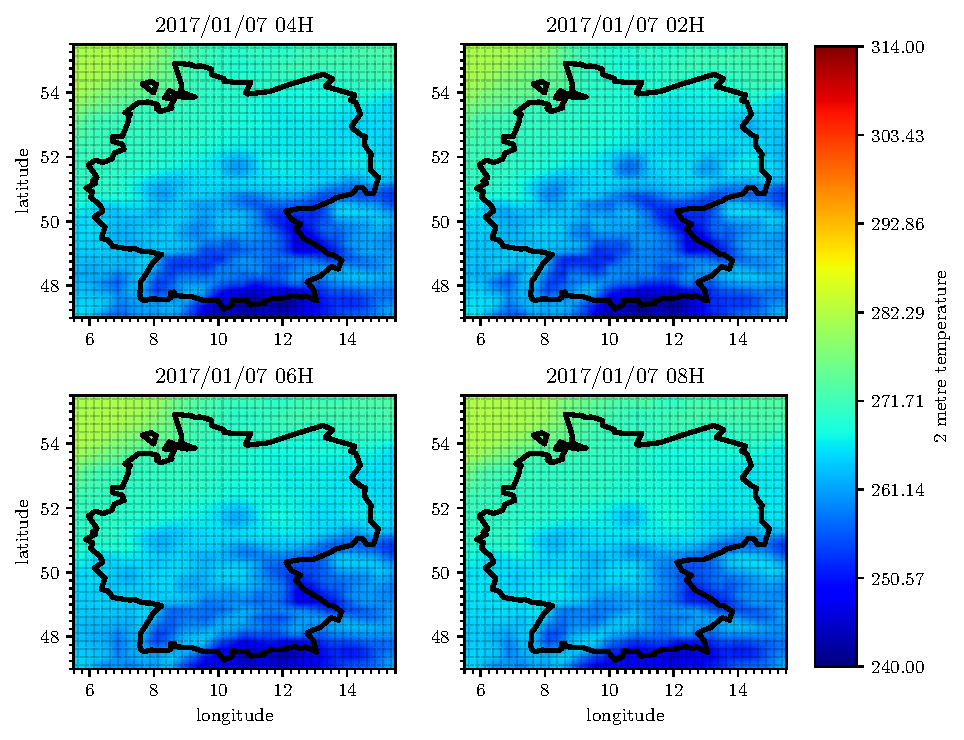
\includegraphics[width=\textwidth]{plots/t2m/bundles/maxvar4_maps}%
\caption{Map showing 4 times with highest temperature variance in germany, where top left is highest, top right second highest, bottom left third highest and bottom right fourth highest variance (TODO put this in text).}%
\label{fig:maxvar4_maps}%
\end{figure}

\begin{figure}[h!]%
\centering
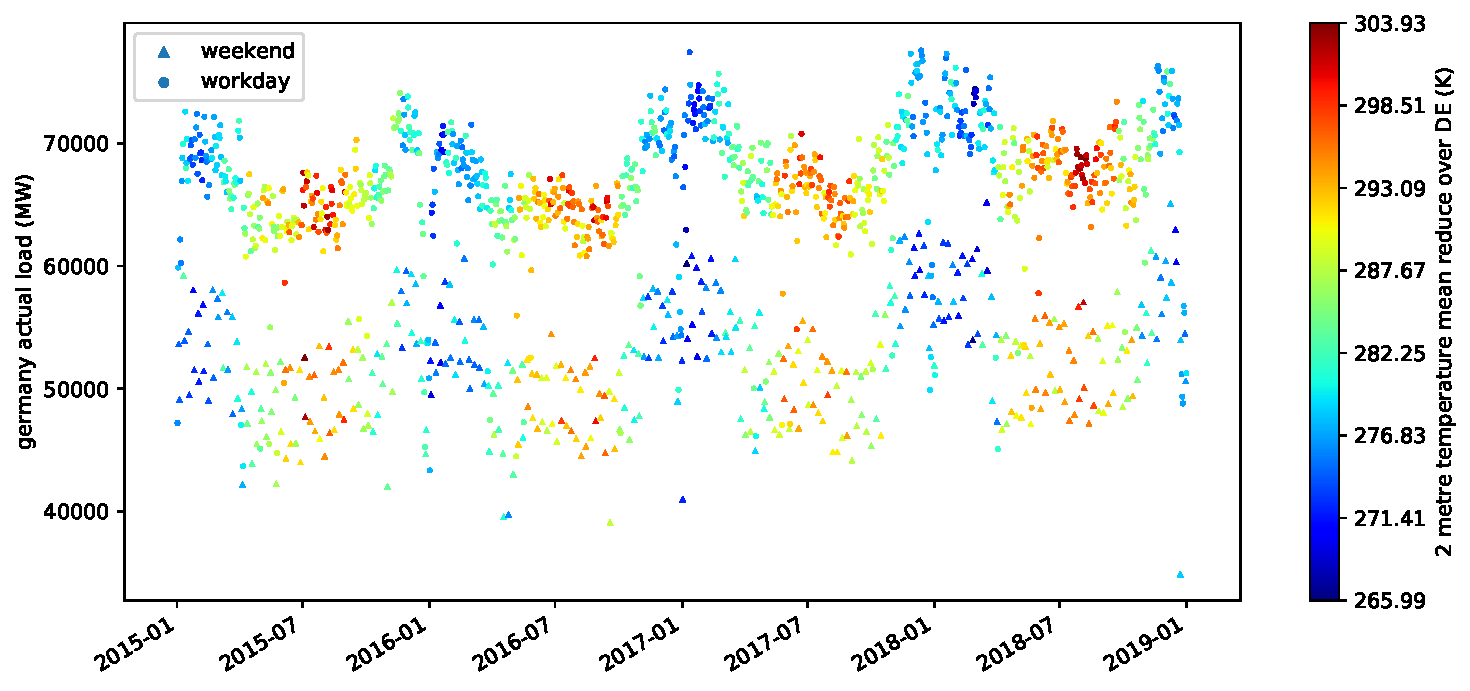
\includegraphics[width=\textheight,angle=-90,origin=c]{plots/t2m_mean_2015010112_2018123112_24F}%
\caption{Load curve with mean of 2 meter height measured temperature in germany as color from 2015/1/1 to 2018/12/31 with one single point per day at 12am utc time respectively.}%
\label{fig:t2m_mean_2015010112_2018123112_24F}%
\end{figure}

\begin{figure}[h!]%
\centering
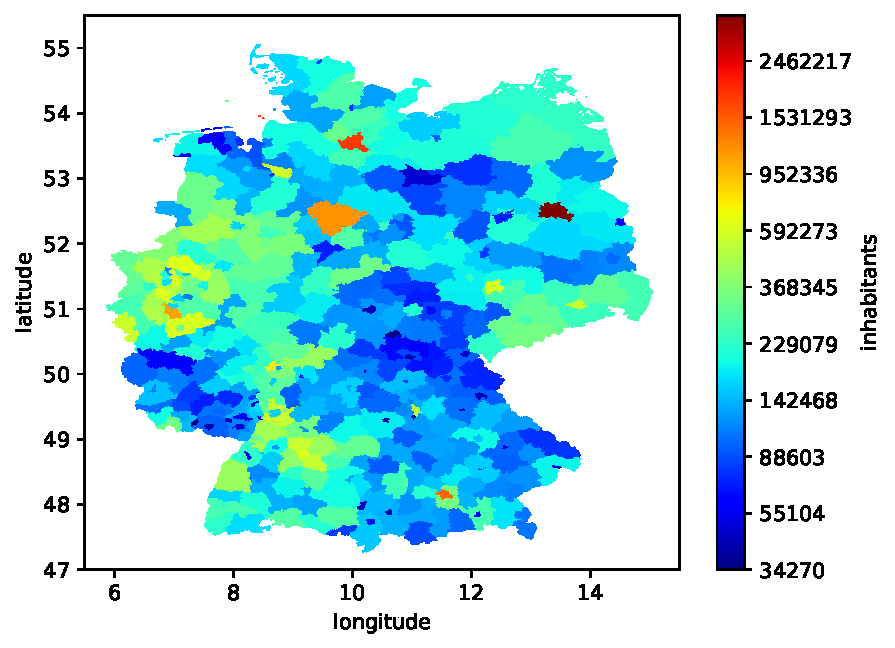
\includegraphics[width=\textwidth]{plots/demo/demo2018_logscale}%
\caption{Population of germany for each region respectively using a log scale for better distinction.}%
\label{fig:demo2018_logscale}%
\end{figure}

\begin{table}[h!]%
\rowcolors{2}{gray!25}{white}
\centering
\footnotesize
\begin{tabular}{llrr}
\tablehead variable name & \tablehead units & \tablehead min & \tablehead max \\\hline
10 metre U wind component & $m~s^{-1}$ & -18.56 & 21.92 \\
10 metre V wind component & $m~s^{-1}$ & -21.51 & 20.00 \\
2 metre temperature & $K$ & 240.97 & 313.26 \\
Leaf area index, high vegetation & $m^{2}~m^{-2}$ & 0.00 & 4.90 \\
Leaf area index, low vegetation & $m^{2}~m^{-2}$ & 0.00 & 3.84 \\
Low cloud cover & $(0~-~1)$ & 0.00 & 1.00 \\
Soil temperature level 1 & $K$ & 257.91 & 313.64 \\
Surface latent heat flux & $J~m^{-2}$ & -2203977.00 & 359411.00 \\
Surface net thermal radiation & $J~m^{-2}$ & -663417.00 & 142945.02 \\
Surface sensible heat flux & $J~m^{-2}$ & -1703159.00 & 801354.00 \\
Total cloud cover & $(0~-~1)$ & 0.00 & 1.00 \\
Total column rain water & $kg~m^{-2}$ & 0.00 & 2.73 \\
Total sky direct solar radiation at surface & $J~m^{-2}$ & -0.12 & 3088320.00 \\
\end{tabular}
\caption[List of exogenous weather variables used to forecast the load including min, max values from \gls{ecmwf}.]{List of exogenous weather variables used to forecast the load including min, max values from \tcite{ecmwf}.}
\label{tab:wvars}
\end{table}


\subsection{Load data}


%Describe the data set you are using. Use appropriate visualization (\eg graphs, statistical summaries \etc) to help the reader get to know your data set.

\Cref{tab:wvars} is an example table. Remember to use full sentences in your caption and explain everything one can see in the table there as well. You can of course also use a simpler format for your table.

%\begin{table}[h!]%
%\caption{Example table with rotated table heads to save space and two different row colours to ease the readability.}
%\rowcolors{2}{gray!25}{white}
%\centering
%\footnotesize
%\begin{tabular}{lll}
%\toprule \noalign{\smallskip}
%\rottblhead{\tablehead Header 1} & \rottblhead{\tablehead Header 2} & \rottblhead{\tablehead Header 3} \\ \midrule
%entry 1 & entry 2 & entry 3 \\ 
%entry 1 & entry 2 & entry 3 \\ 
%entry 1 & entry 2 & entry 3 \\ 	\bottomrule
%\end{tabular}
%\label{tab:example}
%\end{table}


\section{Programming part}
\label{sec:prog}

\subsection{Programming Language}

For the programming part, Python3.6+ has been chosen, as there is a variety of libraries to process all used file formats and because it tends to be a time saving language, also for visualization.\\

\subsection{Documentation}

In regard to coding styles, especially when it comes to docstrings, the numpy conventions were used. The three major points for this were first, that it is a popular and often used style, then it is also a visually oriented style which means, that it is easy to read and last it is supported by several (TODO check which, sphinx?!) autodoc tools that create a HTML based documentation from existing source code with docstrings.\\


\section{Results}
\label{sec:results}

Describe the results you have obtained using your methods described above. Again use proper visualization methods.

\subsection{Experiment 1}

\dots

\subsection{Experiment 2}

\dots
\chapter{Discussion}
\label{ch:discussion}

Considering the main research question of this thesis, whether grid-based weather information does have a benefit on energy forecasting, it is now possible to approach an answer. As already pointed out in \Cref{sec:results}, using the actual grid points themselves does not result in any improvement, but the results rather deteriorate. This seems to suggest that there is no benefit at all, using grid-based data for energy forecasting. However, grid-based data can be very useful when it is being conglomerated or compressed in a representative form, such as the mean over the longitude and latitude. This can also be observed in \Cref{sec:results}, where the averaged 2 metre temperature actually improves the forecast accuracy. The special upside in using grid-based data, such as the data from \gls{ecmwf}, is, that it can be conglomerated over any desired locality as it is available for most locations. This allows it to be used for forecasts at arbitrary locations. Though, from the missing results to most of the given weather variables, it is can not be said which of them are most suitable to be used as inputs for energy forecasting. This provides an interesting subject for further research. But also other methods could be considered for further research, like filtering grid points by economic activity. Another possibility would be to use completely different models such as \gls{rnn}, which are particularly suitable for time series forecasting.\\
%outlook: try other methods to compress the data as representative as possible, mean over highest populated regions, or regions filtered by economic activity also compressed or so
%Looking at the results from \Cref{sec:results}, 

%This chapter is supposed to discuss your results. Point out what your results mean.
%What are the limitations of your approach, managerial implications or future impact?
%
%Explain the broader picture but be critical with your methods.
\chapter{Conclusion}
\label{ch:Conclusion}

Repeat the problem and its relevance, as well as the contribution (plus quantitative results). 
Look back at what you have written in the introduction.

Provide an outlook for further research steps.


%% ----------------
%% |   Glossary   |
%% ----------------

\printglossary[title=Terms and abbreviations,toctitle=Terms and abbreviations,type=\acronymtype]


%% --------------------
%% |   Bibliography   |
%% --------------------

%% Add entry to the table of contents for the bibliography
\printbibliography[heading=bibintoc]

%% ----------------
%% |   Appendix   |
%% ----------------
\appendix
%% LaTeX2e class for student theses
%% appendix
%% 
%% Based on SDQ KIT Template by Erik Burger
%%
%% Karlsruhe Institute of Technology
%% Institute for Automation and Applied Informatics
%% AIDA Research Group
%%
%% Nicole Ludwig
%% nicole.ludwig@kit.edu
%%
%% Version 1.2, 2018-10-11


\iflanguage{english}
{\chapter{Appendix}}    % english style
{\chapter{Anhang}}      % german style
\label{chap:appendix}


%% -------------------
%% | Example content |
%% -------------------
\section{First Section}
\label{sec:appendix:FirstSection}

\dots

\begin{figure}[h!]%
\centering
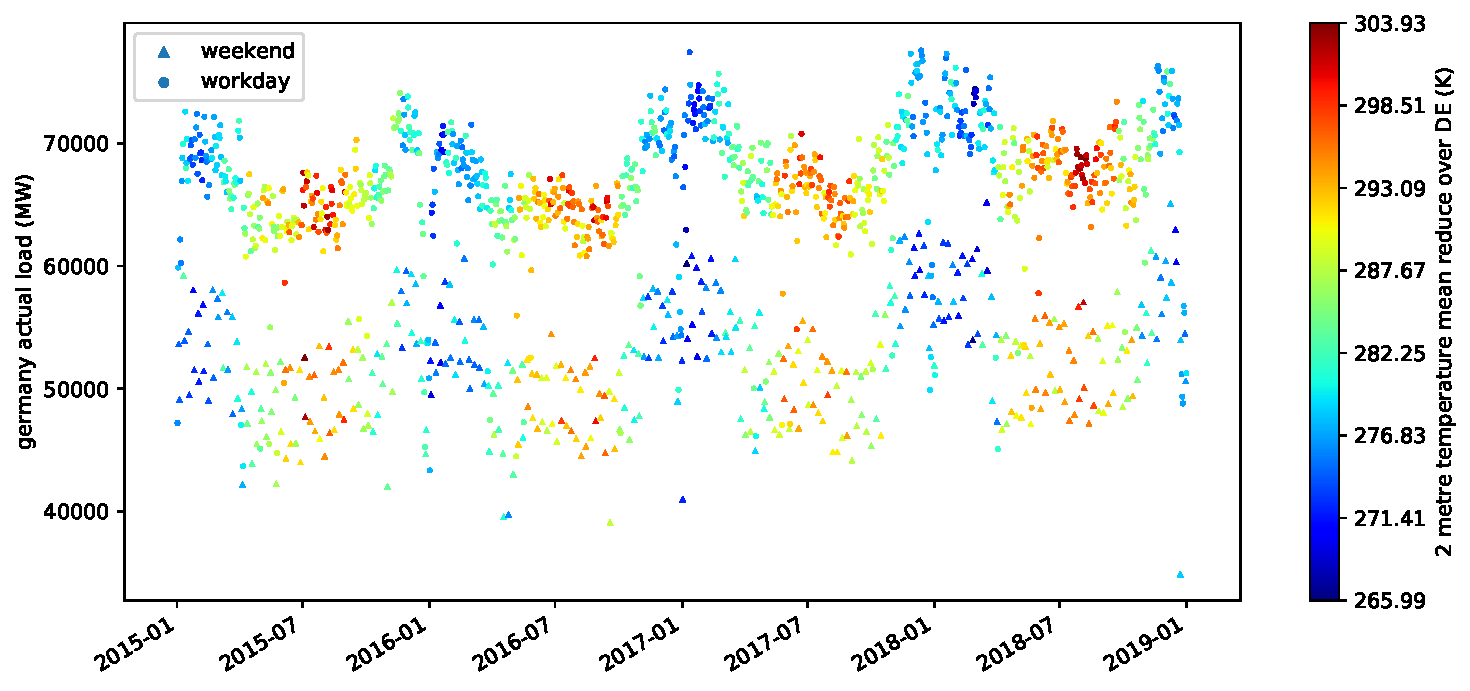
\includegraphics[width=\textheight,angle=-90,origin=c]{plots/t2m_mean_2015010112_2018123112_24F}%
\caption{Load curve with mean of 2 meter height measured temperature in germany as color from 2015/1/1 to 2018/12/31 with one single point per day at 12am utc time respectively.}%
\label{fig:t2m_mean_2015010112_2018123112_24F}%
\end{figure}
		
%\setcounter{figure}{0}
%		
%\begin{figure} [ht]
%  \centering
%  \caption{A figure}
%  \label{fig:anotherfigure}
%\end{figure}


\end{document}